%\documentclass[paper]{geophysics}
\documentclass[paper,revised]{geophysics}
\usepackage{cleveref} %for cref

% An example of defining macros
\newcommand{\rs}[1]{\mathstrut\mbox{\scriptsize\rm #1}}
\newcommand{\rr}[1]{\mbox{\rm #1}}

\begin{document}

\title{An example \emph{Geophysics} article, \\ with a two-line title}

\renewcommand{\thefootnote}{\fnsymbol{footnote}} 

\ms{GEO-Example} % paper number

\address{
\footnotemark[1]BP UTG, \\
200 Westlake Park Blvd, \\
Houston, TX, 77079 \\
\footnotemark[2]Bureau of Economic Geology, \\
John A. and Katherine G. Jackson School of Geosciences \\
The University of Texas at Austin \\
University Station, Box X \\
Austin, TX 78713-8924}
\author{Joe Dellinger\footnotemark[1] and Sergey Fomel\footnotemark[2]}

\footer{Example}
\lefthead{Dellinger \& Fomel}
\righthead{\emph{Geophysics} example}

\maketitle

\begin{abstract}
  This is an example of using \textsf{geophysics.cls} for writing
  \emph{Geophysics} papers.
\end{abstract}

\section{Introduction}

The nonlinear relation between the physical properties of earth and natural phenomina expalin the wave behaviour is responsible for FWI to stuck in local minima if the starting model is not lie within the basin of attraction. in this both are used together because both have advantages and disadvantages global is best in exploration and local is best in exploitation. PSO is easily parallelized.
Some of the appealing facts of PSO are its convenience, simplicity and easiness of implementation requiring.
The prominent features of PSO are its easy implementation, robustness to control parameters and computation efficiency compared with other existing heuristic algorithms such as genetic algorithm in a continuous problem.
method \ref{method}
\section{Methodology}
\label{method}
This approach involves two steps. First, a coarse velocity model is prepared using PSO by optimizing the depth, interface velocity, and the rate of change of velocity between interfaces. This model serves as an initial model for conventional gradient-based FWI in the second step.
\subsection{Particle Swarm Optimization}
Particle Swarm Optimization (PSO) is a stochastic method developed by James Kennedy and Russell Eberhart in 1995. Inspired by the social behavior of birds flocking to find food, they formulated a mathematical model to simulate this behavior. This model is widely applied to solve various optimization problems. They identified that the fundamental principle guiding birds' food-finding behavior is their ability to communicate with each other. Each bird in the process knows its current position \((x_i(t))\) and best position \((p_i(t))\), determined by evaluating the fitness using a cost function. Additionally, each bird shares its best position with others, contributing to the collective knowledge of the flock's best position \((g(t))\). Each bird's next movement is adjusted by its own best, the flock's best, and its current position. This iterative process continues at each step, ultimately converging towards a globally optimal position through the collaborative effort of all birds.This natural phenomenon is mathematically described by the velocity update equation \ref{eqn:pso_1} and the position update equation \ref{eqn:pso_2}.
\begin{itemize}
	\item \( \mathbf{x}_i(t) \) be the position of particle \( i \) at iteration \( t \).
	\item \( \mathbf{v}_i(t) \) be the velocity of particle \( i \) at iteration \( t \).
	\item \( \mathbf{p}_i(t) \) be the personal best position of particle \( i \) until iteration \( t \).
	\item \( \mathbf{g}(t) \) be the global best position among all particles until iteration \( t \).
	\item \( w \) be the inertia weight.
	\item \( c_1 \) and \( c_2 \) be the cognitive and social acceleration coefficients, respectively.
	\item \( r_1 \) and \( r_2 \) be random numbers uniformly distributed in the range \([0, 1]\).
\end{itemize}

The velocity and position update rules for each particle are given by:
\begin{equation}	
	\mathbf{v}_i(t+1) = w \mathbf{v}_i(t) + c_1 r_1 (\mathbf{p}_i(t) - \mathbf{x}_i(t)) + c_2 r_2 (\mathbf{g}(t) - \mathbf{x}_i(t))	
	\label{eqn:pso_1}
\end{equation}

\begin{equation}	
	\mathbf{x}_i(t+1) = \mathbf{x}_i(t) + \mathbf{v}_i(t+1)	
	\label{eqn:pso_2}
\end{equation}

Where:
\begin{itemize}
	\item \( w \) controls the influence of the previous velocity (inertia).
	\item \( c_1 \) and \( c_2 \) represent the trust of the particle in itself and in the swarm, respectively.
	\item \( r_1 \) and \( r_2 \) introduce stochasticity to the particle's movement.
\end{itemize}
\subsection{Optimization Parameters}
The updates in the Particle Swarm Optimization (PSO) algorithm are influenced by several controlling parameters, including the inertia weight \((w)\), acceleration coefficients \((c_1\) and \(c_2)\), population size of the swarm, and the number of iterations. Among these, the inertia weight is the most critical tuning parameter as it balances the exploration and exploitation capabilities of PSO by adjusting the contribution of the particle's previous velocity. An inertia weight value between 0.4 and 0.9 is generally found to provide good convergence. The cognitive and social coefficients \((c_1\) and \(c_2)\) represent the confidence in a particle's own best position and the swarm's best position, respectively, and they influence the updated velocity of the particles. The number of particles in the swarm also affects convergence; as the number of particles increases, the search space expands, potentially leading to better convergence. Experimental studies have shown that a swarm size of around 30 particles is generally effective for finding solutions within optimal iterations. The number of iterations, as with all iterative optimization algorithms, significantly impacts the performance of PSO.
\\
This contribution of different parameters for succes of PSO make it is necessary to decide the combination of these parameters precisely. we have performed experiments to find the optimal combination of this values, for these experiment we have choose four nonlinear functions Ackley, Griewank, Rastrigin, and Styblinski-Tang function shown in figure \ref{fig:ackley}, \ref{fig:griewank}, \ref{fig:rastrigin}, and \ref{fig:styblinski} respectively. These experiments are performed to determine the optimal value of the optimization coefficient and examine the relationship between the number of iterations and swarm size. Since both swarm size and iteration count impact computational time, it is essential to balance these factors to achieve effective optimization while minimizing computational costs. To fairly compare the effects of swarm size and the number of iterations, the rate of increase for both parameters is kept consistent. Following this, PSO is applied to the Schwefel function using the parameters chosen from the previous experiment to achieve the parameters that lead to the best convergence. To analyze performance, accuracy is evaluated based on the maximum deviation using equation \ref{eqn:accuracy}. Further details of these experiments are outlined below.
\begin{equation}
	Accuracy (\%) = 100 - \left| \frac{optimal \ value - evaluated \ value}{optimal \ value - maximum \ deviation} \right| \times 100
	\label{eqn:accuracy}
\end{equation}
Where:
\begin{itemize}
	\item \(Optimal \  value\), best possible value of the objective function.
	\item \(Evaluated \ value\), value of the objective function at a given point in the feasible domain.
	\item \(Maximum \ deviation\), largest difference between the optimized value and the actual values.
\end{itemize}
\begin{enumerate}
	\item Accuracy with Parameters: In this experiment, optimization is conducted for all specified test functions using varying values of \(c_1\), \(c_2\), and inertia weights, as illustrated in figures \ref{fig:acc_ackley}, \ref{fig:acc_griewank}, \ref{fig:acc_rastrigin}, and \ref{fig:acc_styblinski}. To address the inherent randomness of this stochastic method, we perform 50 runs with 1000 iterations and calculate the average of these results as the final optimized values. 
%\begin{figure}	
%	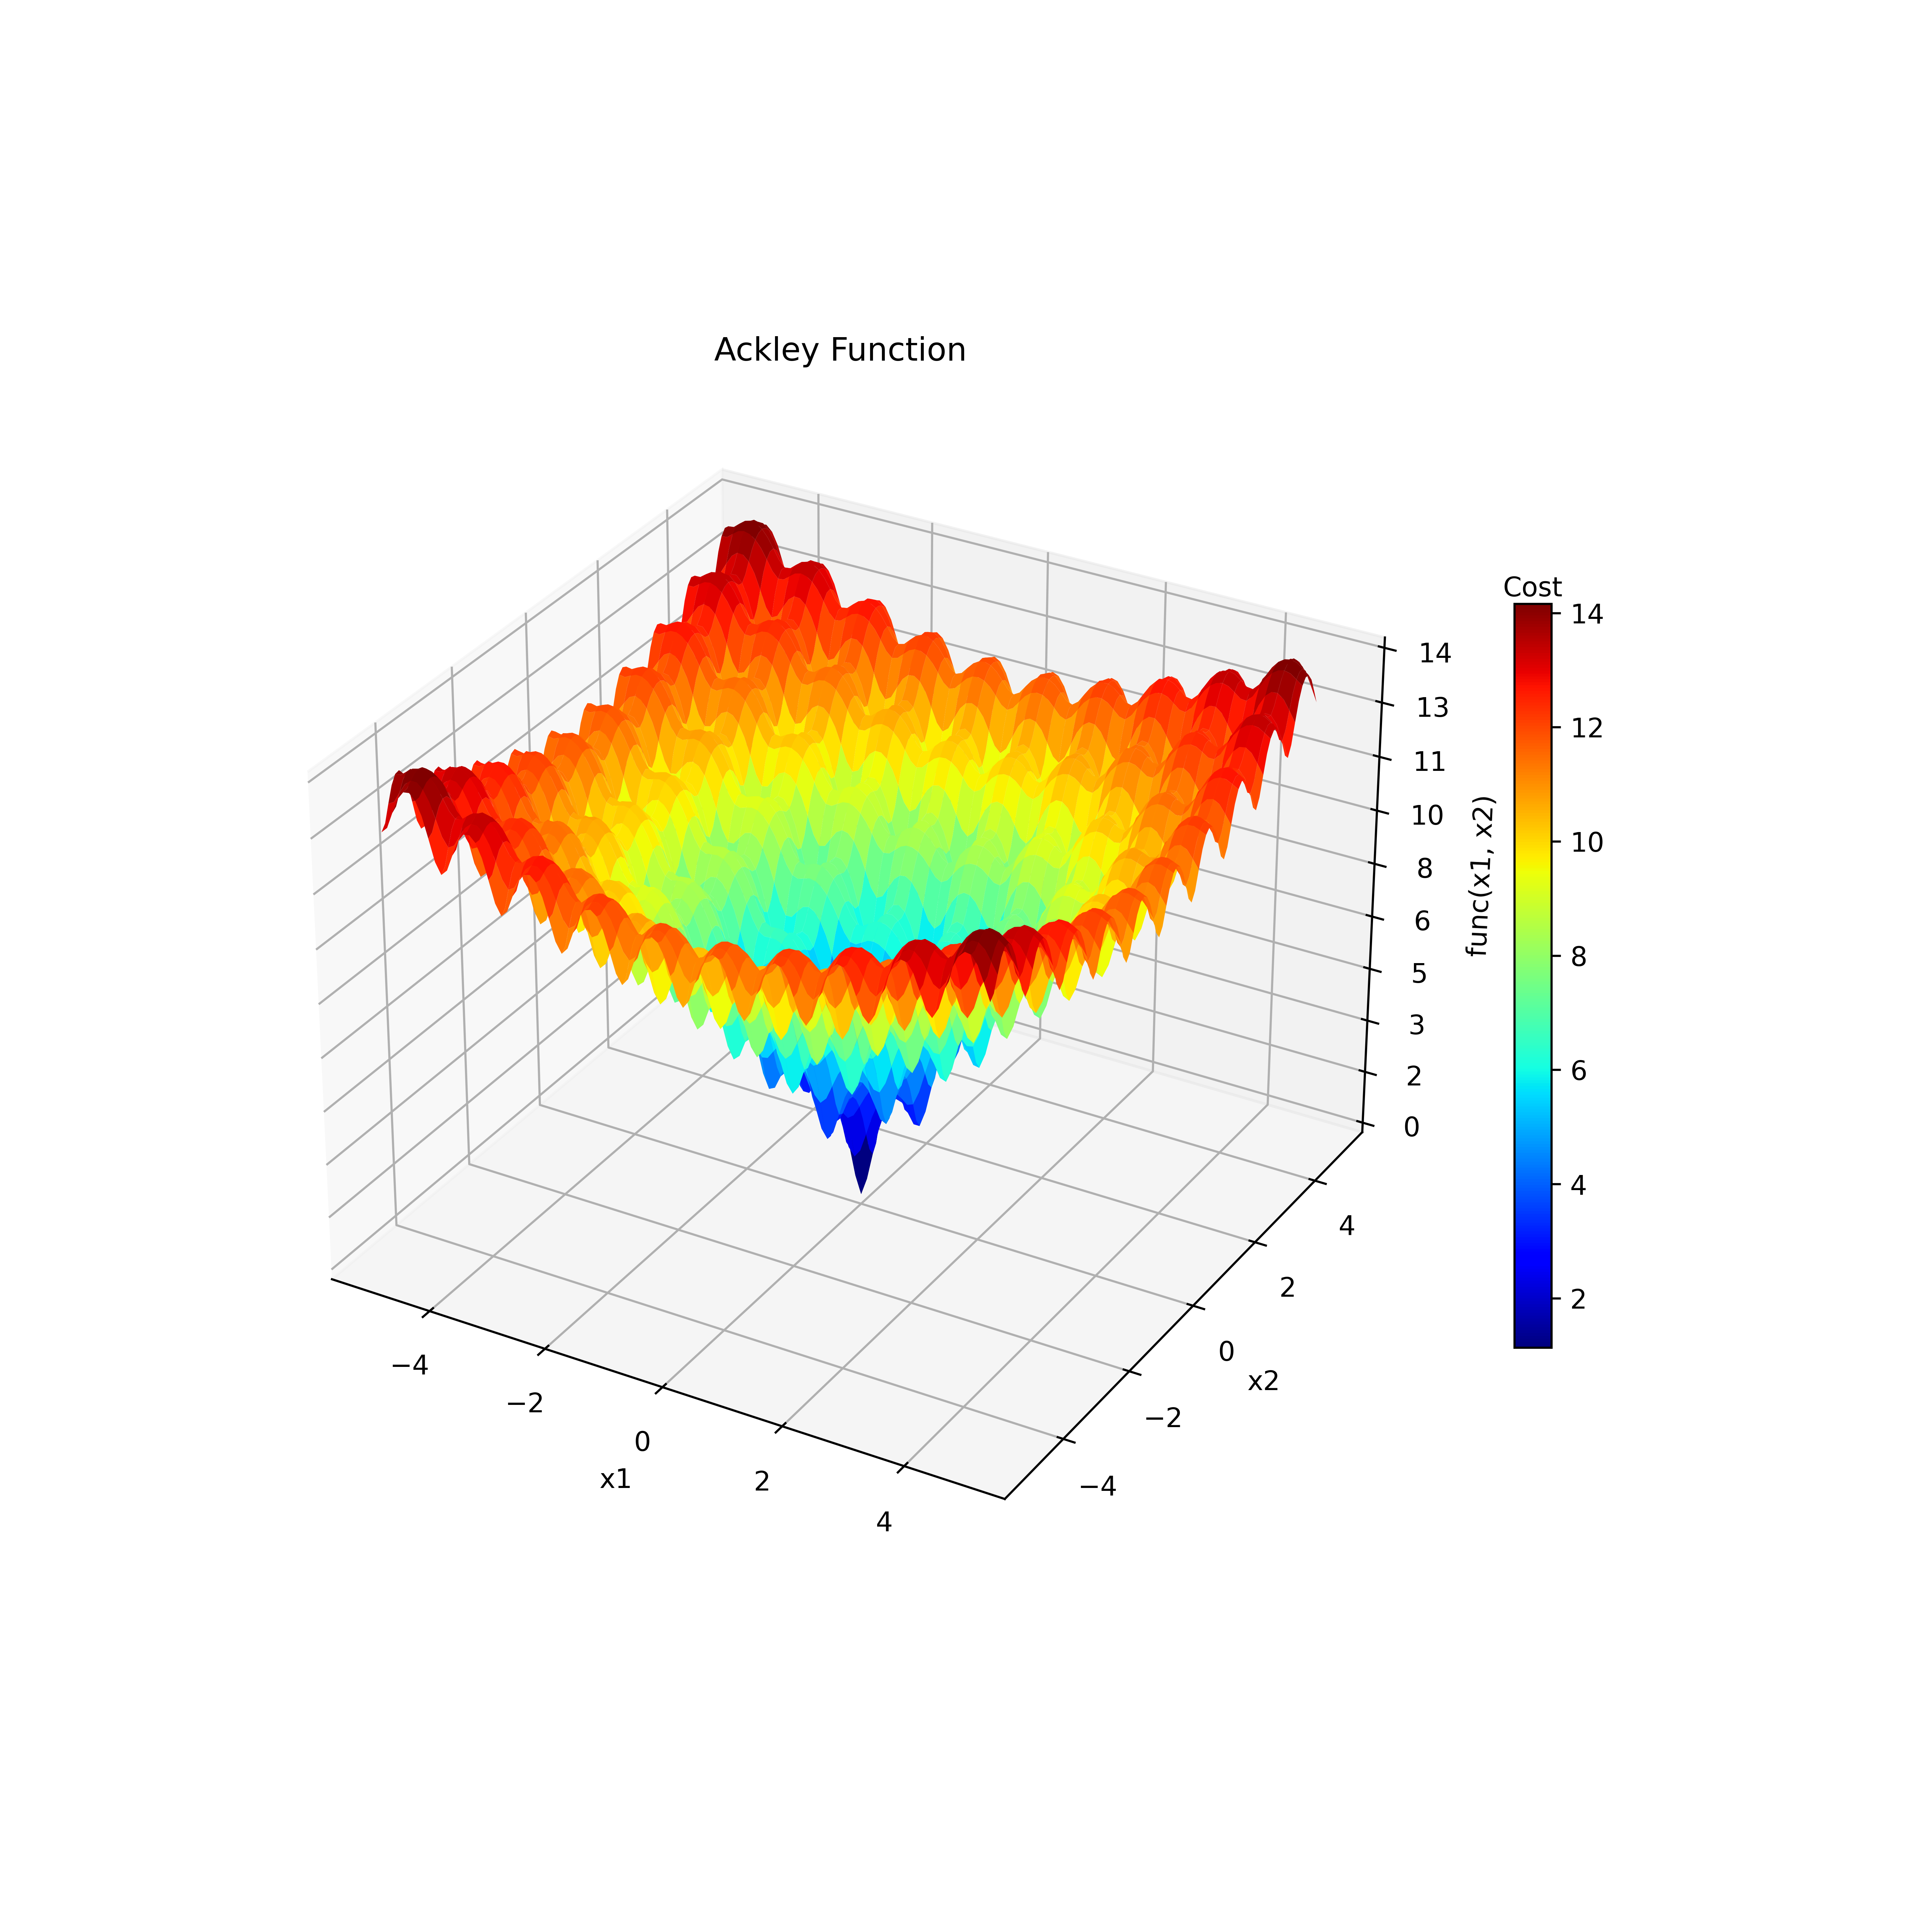
\includegraphics[width=\paperwidth]{Fig/ackley.png}
%	\caption{Ackley function.}
%	\label{fig:ackley}
%\end{figure} 
%\begin{figure}	
%	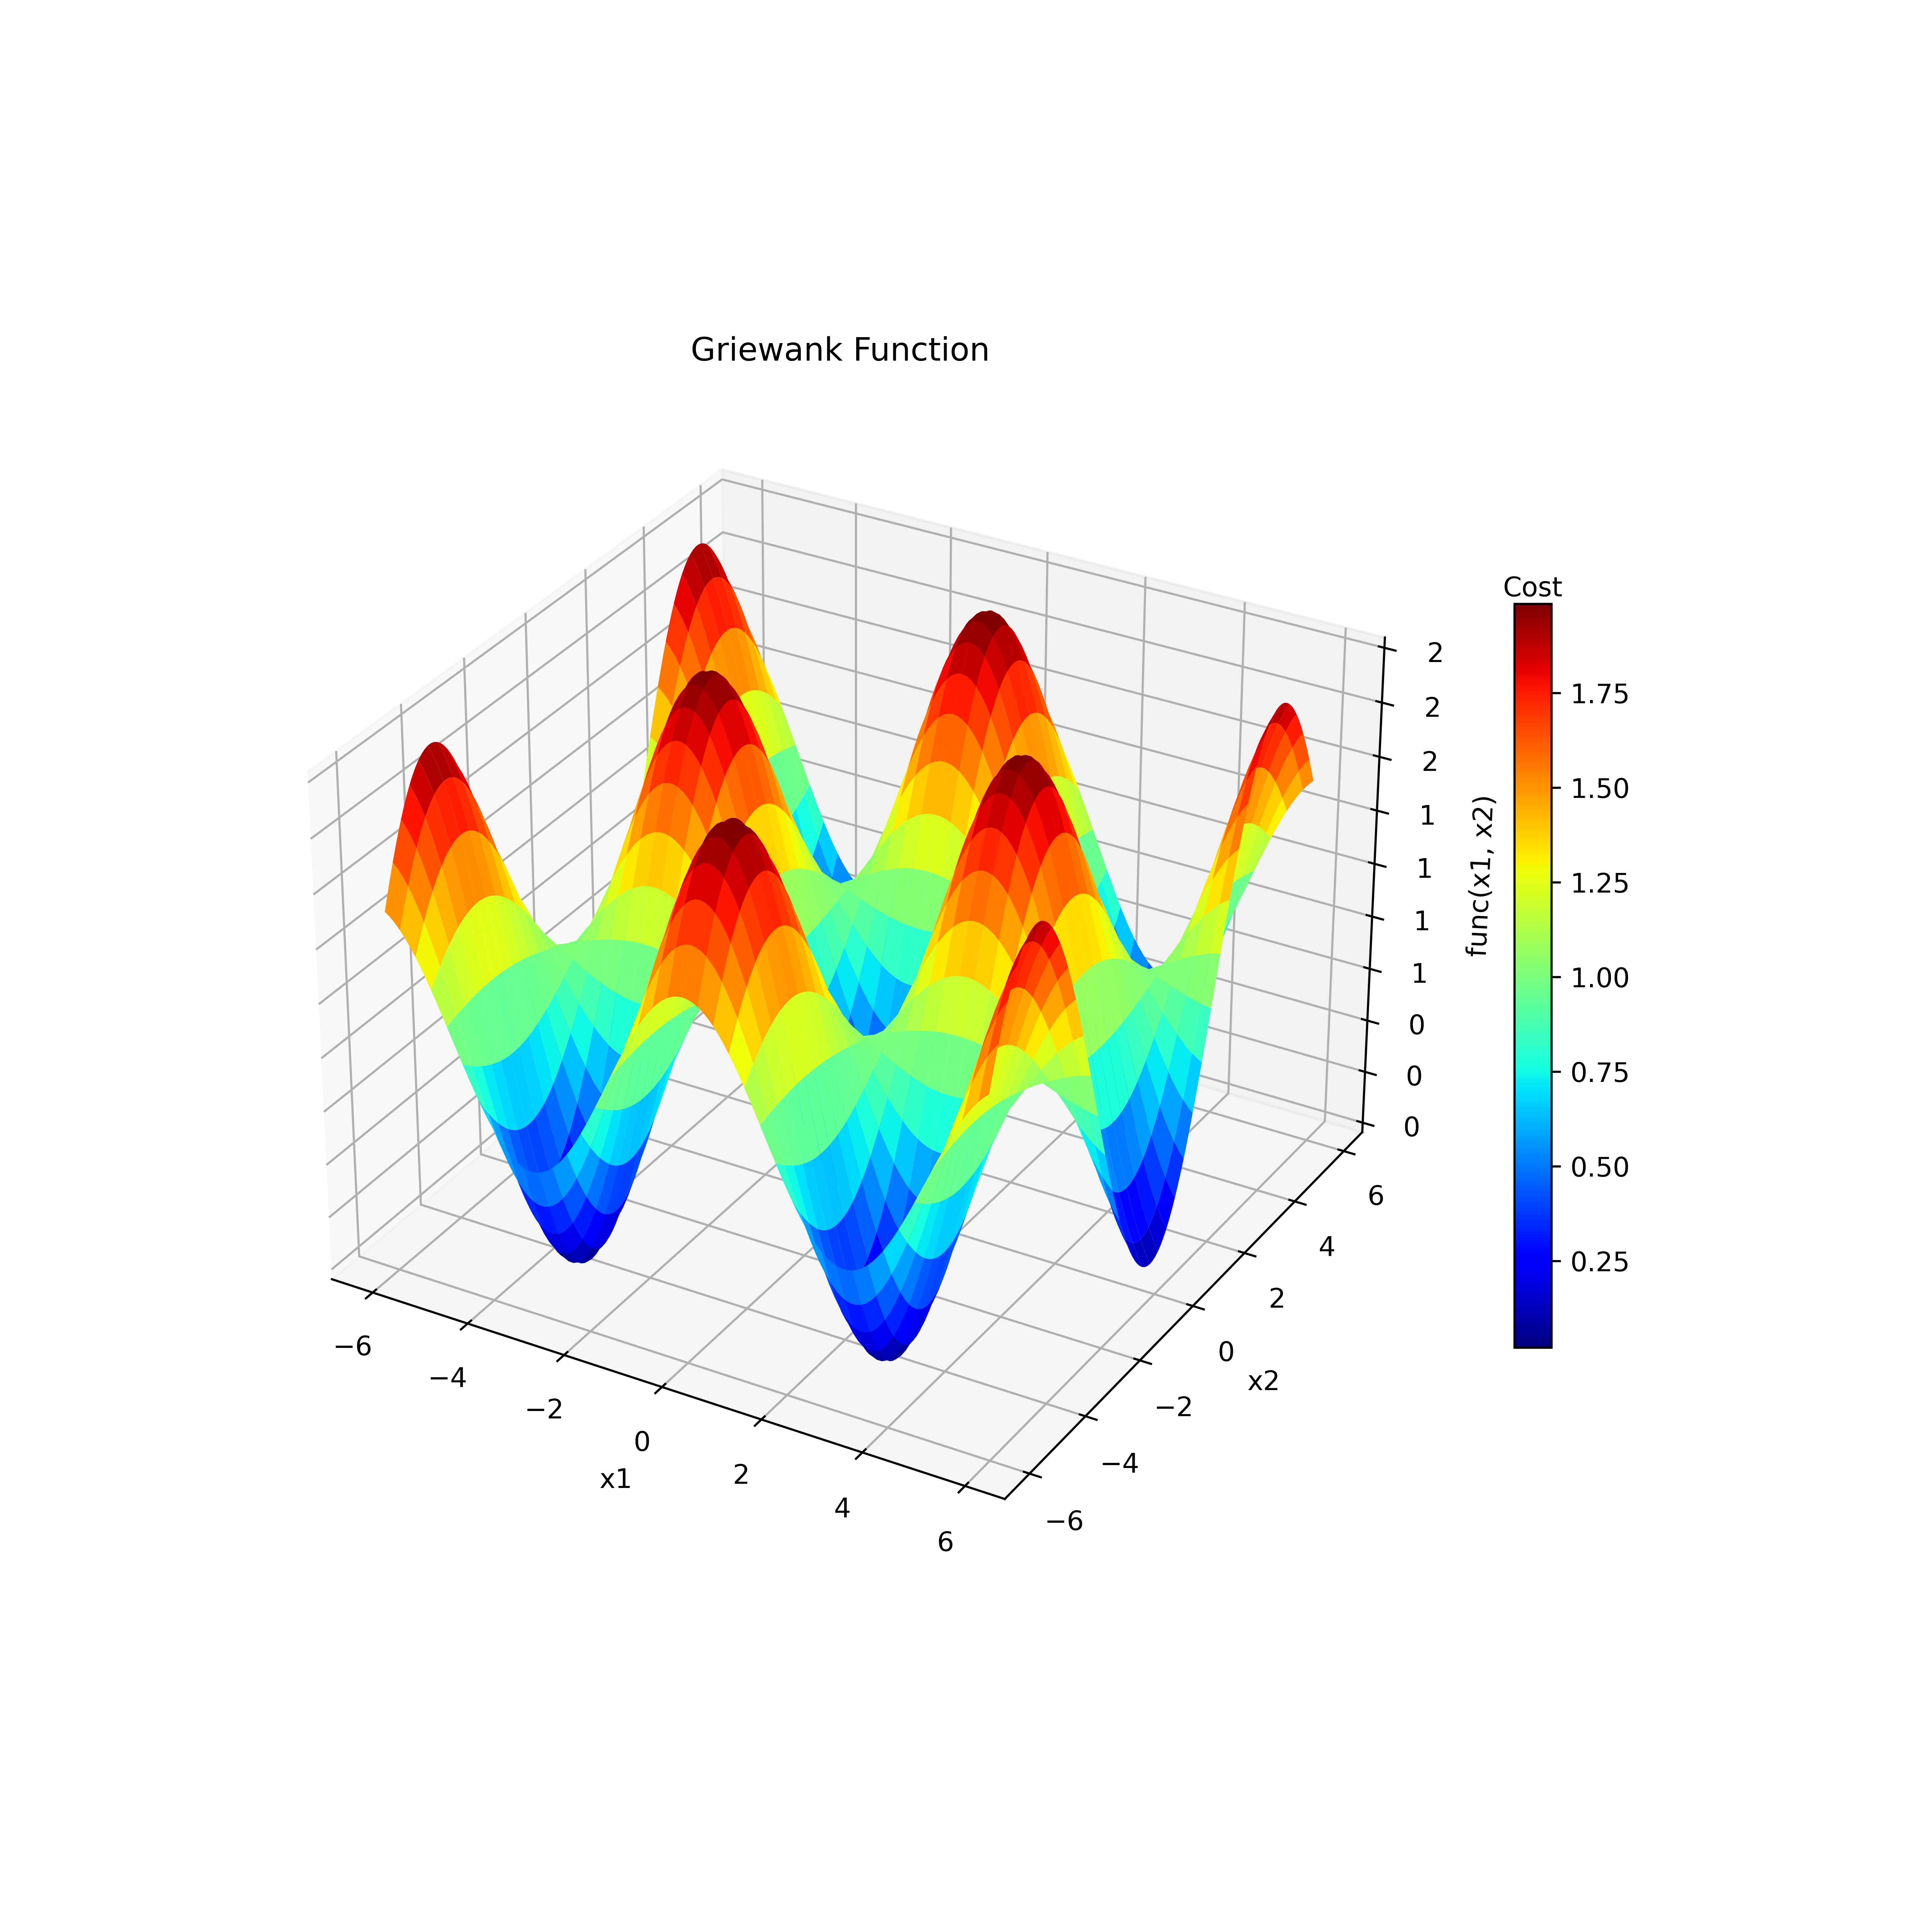
\includegraphics[width=\paperwidth]{Fig/griewank.png}
%	\caption{Griewank function.}
%	\label{fig:griewank}
%\end{figure}
%\begin{figure}	
%	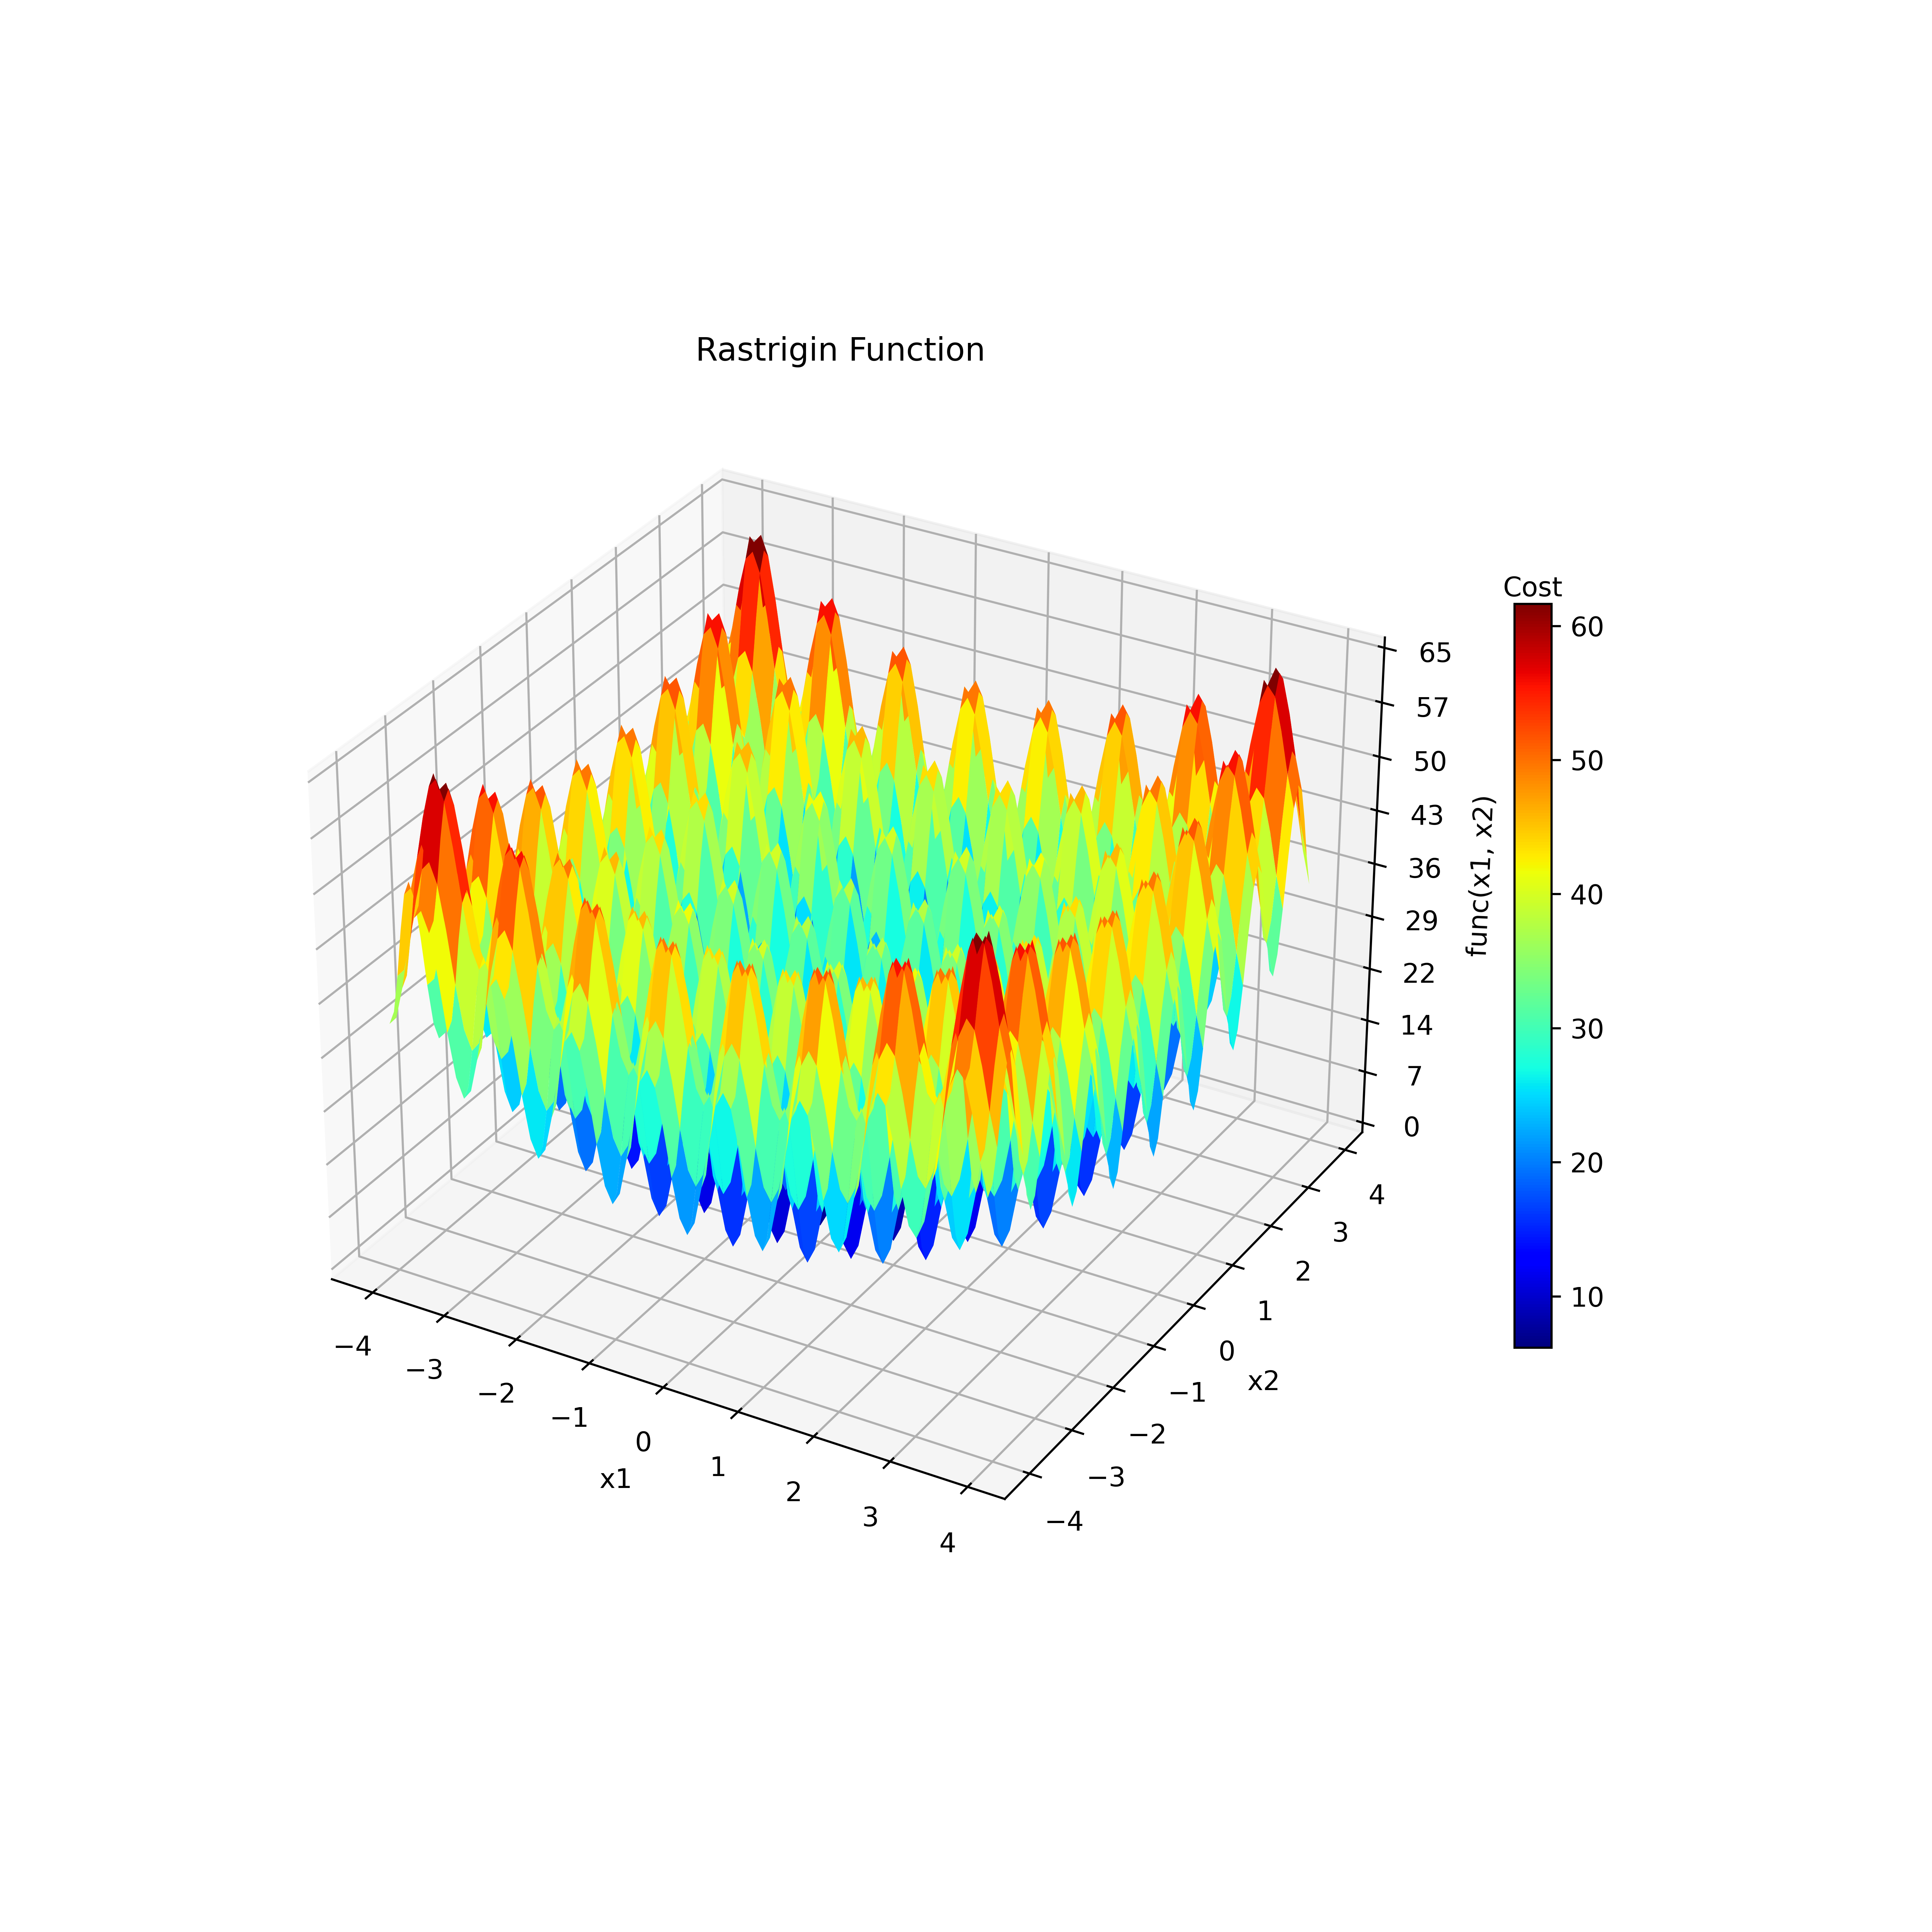
\includegraphics[width=\paperwidth]{Fig/rastrigin.png}
%	\caption{Rastrigin function.}
%	\label{fig:rastrigin}
%\end{figure}
%\begin{figure}	
%	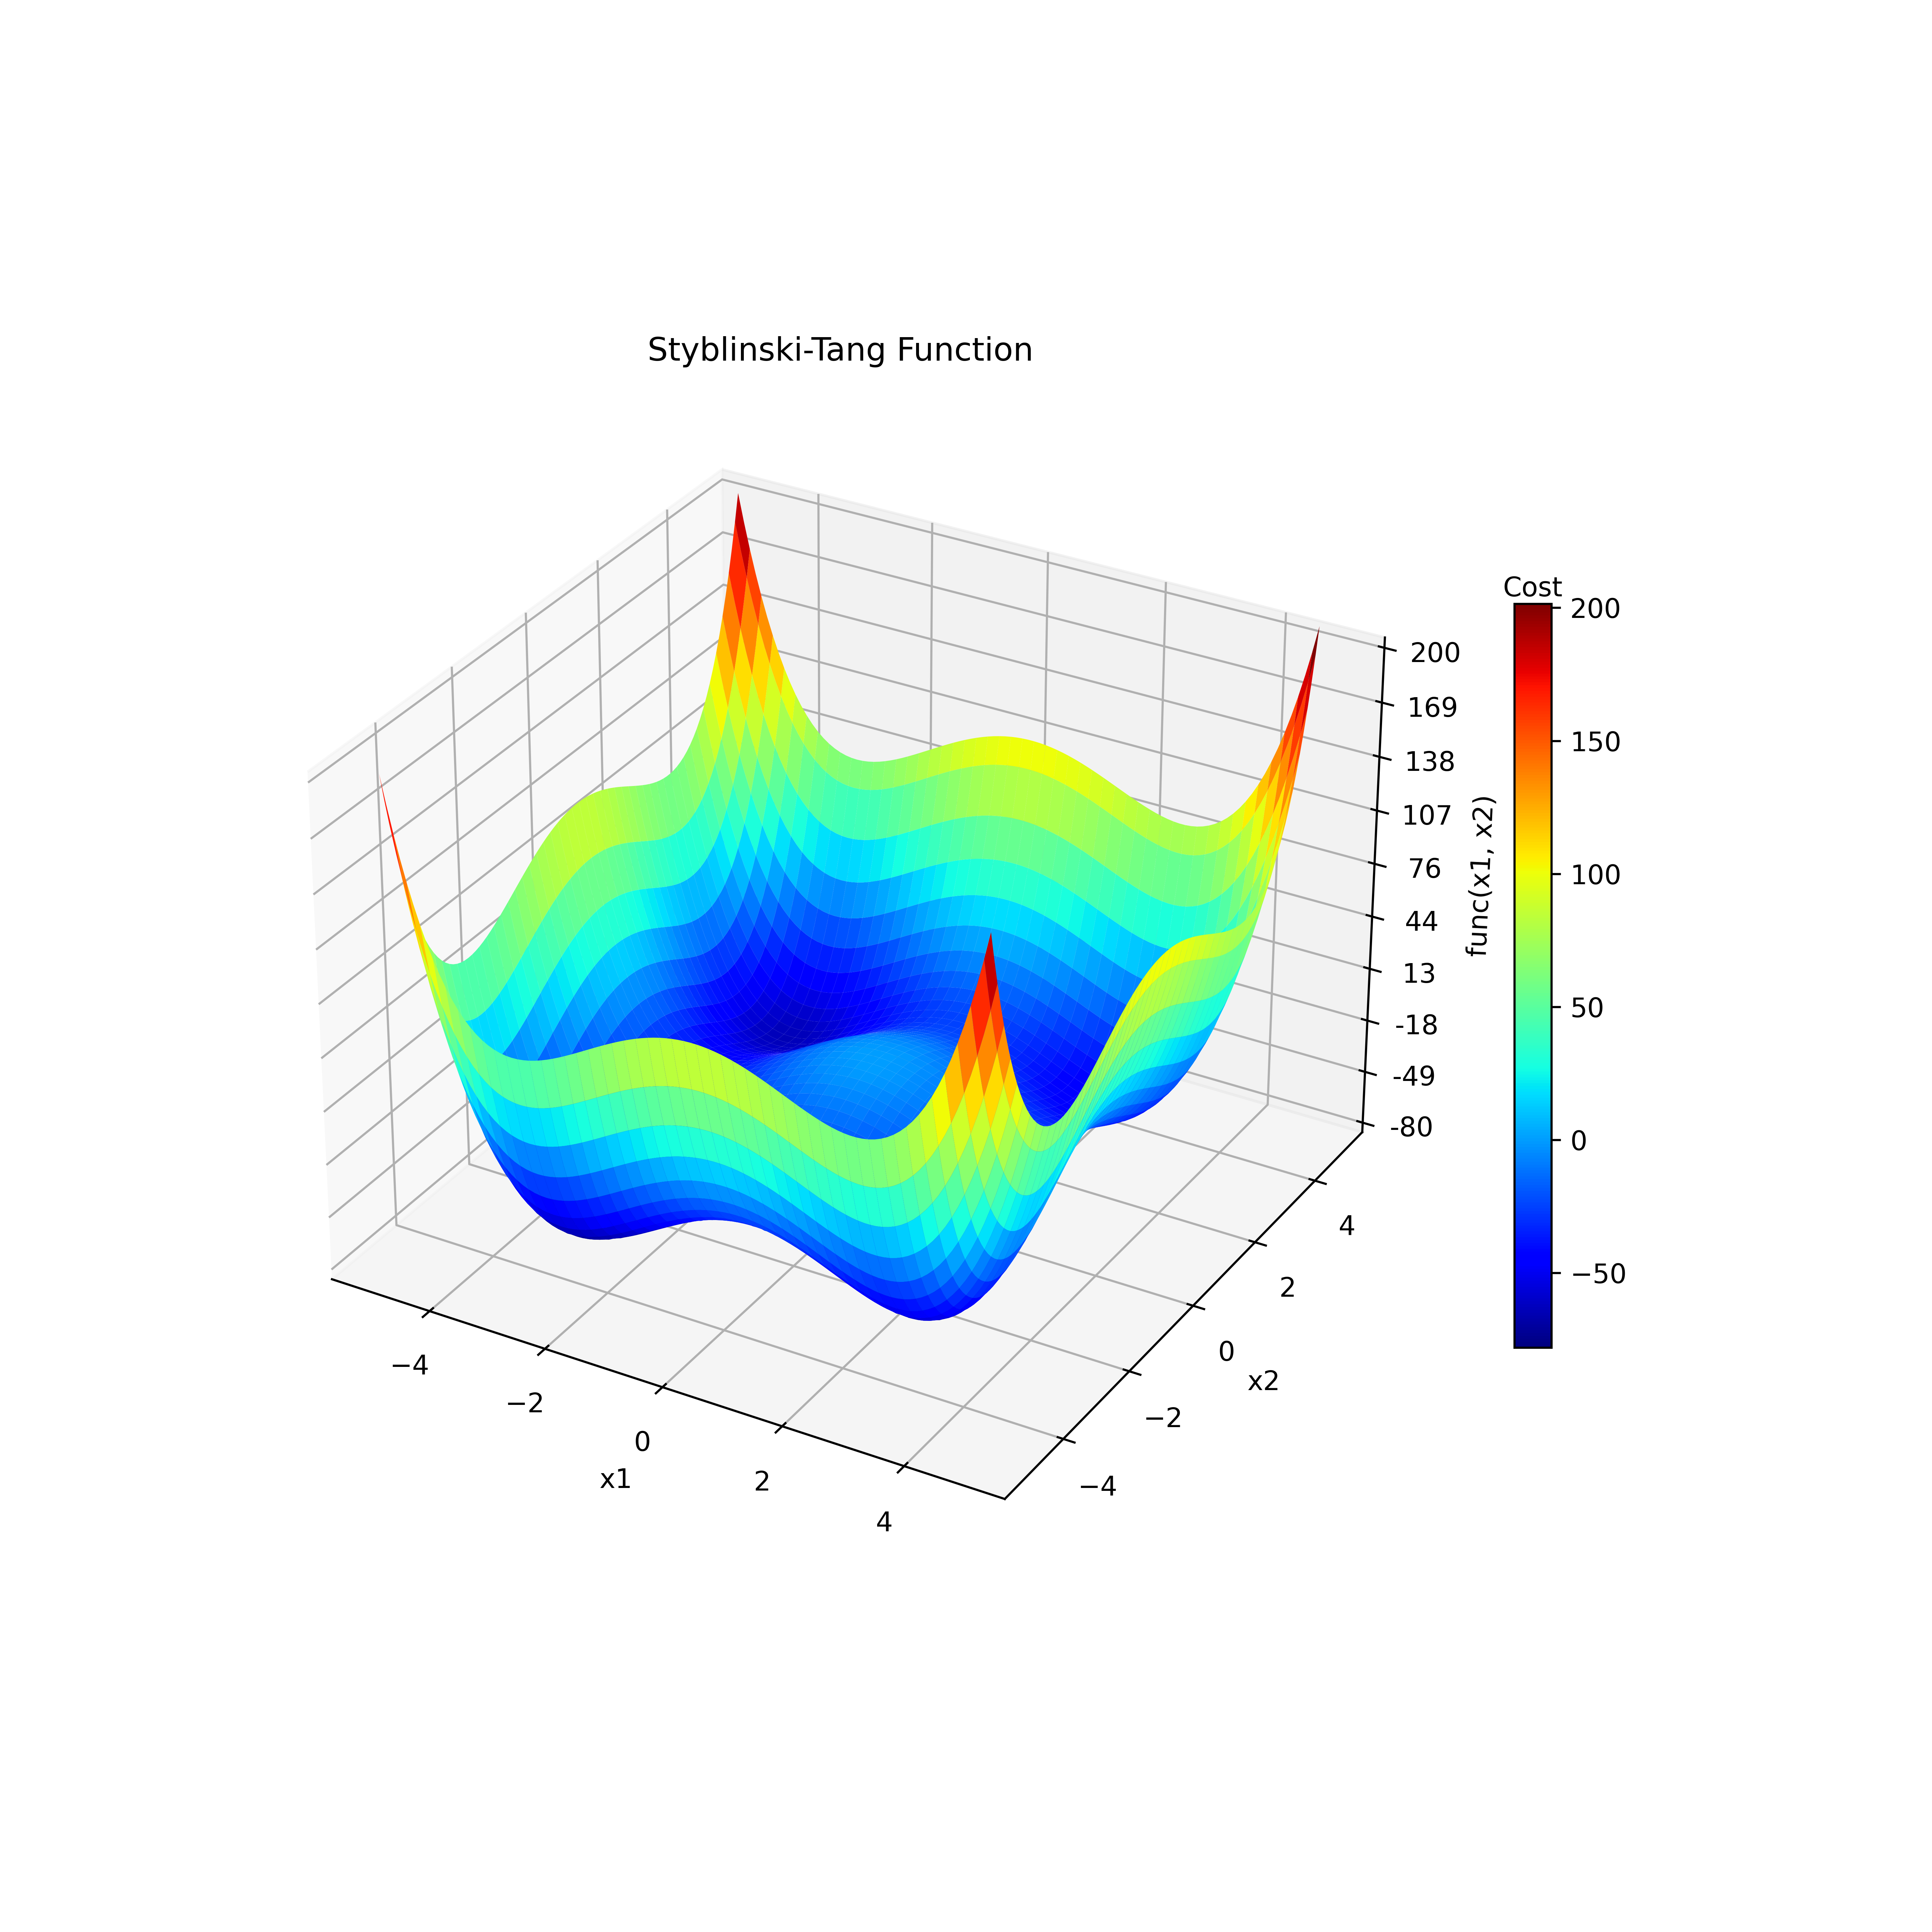
\includegraphics[width=\paperwidth]{Fig/styblinski.png}
%	\caption{Styblinski-Tang function.}
%	\label{fig:styblinski}
%\end{figure}
	
This experiment concludes that a combination of inertia weights between 0.5 and 0.8, \(c_1\) values ranging from 0.6 to 2.0, and \(c_2\) values between 0.6 and 1.8 results in improved accuracy. 
%	\begin{sidewaysfigure}	
%		\includegraphics[width=\paperwidth]{Fig/ackley_para_vs_accuracy.jpeg}
%		\caption{Optimization of the Ackley function with varying inertia weights, \(c_1\), and \(c_2\) coefficients.}
%		\label{fig:acc_ackley}
%	\end{sidewaysfigure} 
%	\begin{sidewaysfigure}	
%		\includegraphics[width=\paperwidth]{Fig/griewank_para_vs_accuracy.jpeg}
%		\caption{Optimization of the Griewank function with varying inertia weights, \(c_1\), and \(c_2\) coefficients.}
%		\label{fig:acc_griewank}
%	\end{sidewaysfigure} 
%	\begin{sidewaysfigure}	
%		\includegraphics[width=\paperwidth]{Fig/rastrigin_para_vs_accuracy.jpeg}
%		\caption{Optimization of the Rastrigin function with varying inertia weights, \(c_1\), and \(c_2\) coefficients.}
%		\label{fig:acc_rastrigin}
%	\end{sidewaysfigure} 
%	\begin{sidewaysfigure}	
%		\includegraphics[width=\paperwidth]{Fig/styblinski_para_vs_accuracy.jpeg}
%		\caption{Optimization of the Styblinski-Tang function with varying inertia weights, \(c_1\), and \(c_2\) coefficients.}
%		\label{fig:acc_styblinski}
%	\end{sidewaysfigure} 

	\item Accuracy with iterations: Here, accuracy is assessed while maintaining a constant swarm size of 30 and an initial iteration count of 1000, which is then increased by factors of 1.67, 2.0, 2.67, 3.00, 5, and 10, to examine how the number of iterations impacts accuracy across all test functions. The results indicate that as the number of iterations increases, accuracy improves, reaching a maximum close to 100 \% when iterations are increased to 10 times, as illustrated in figure \ref{fig:acc_itr}.
%	\begin{figure}	
%		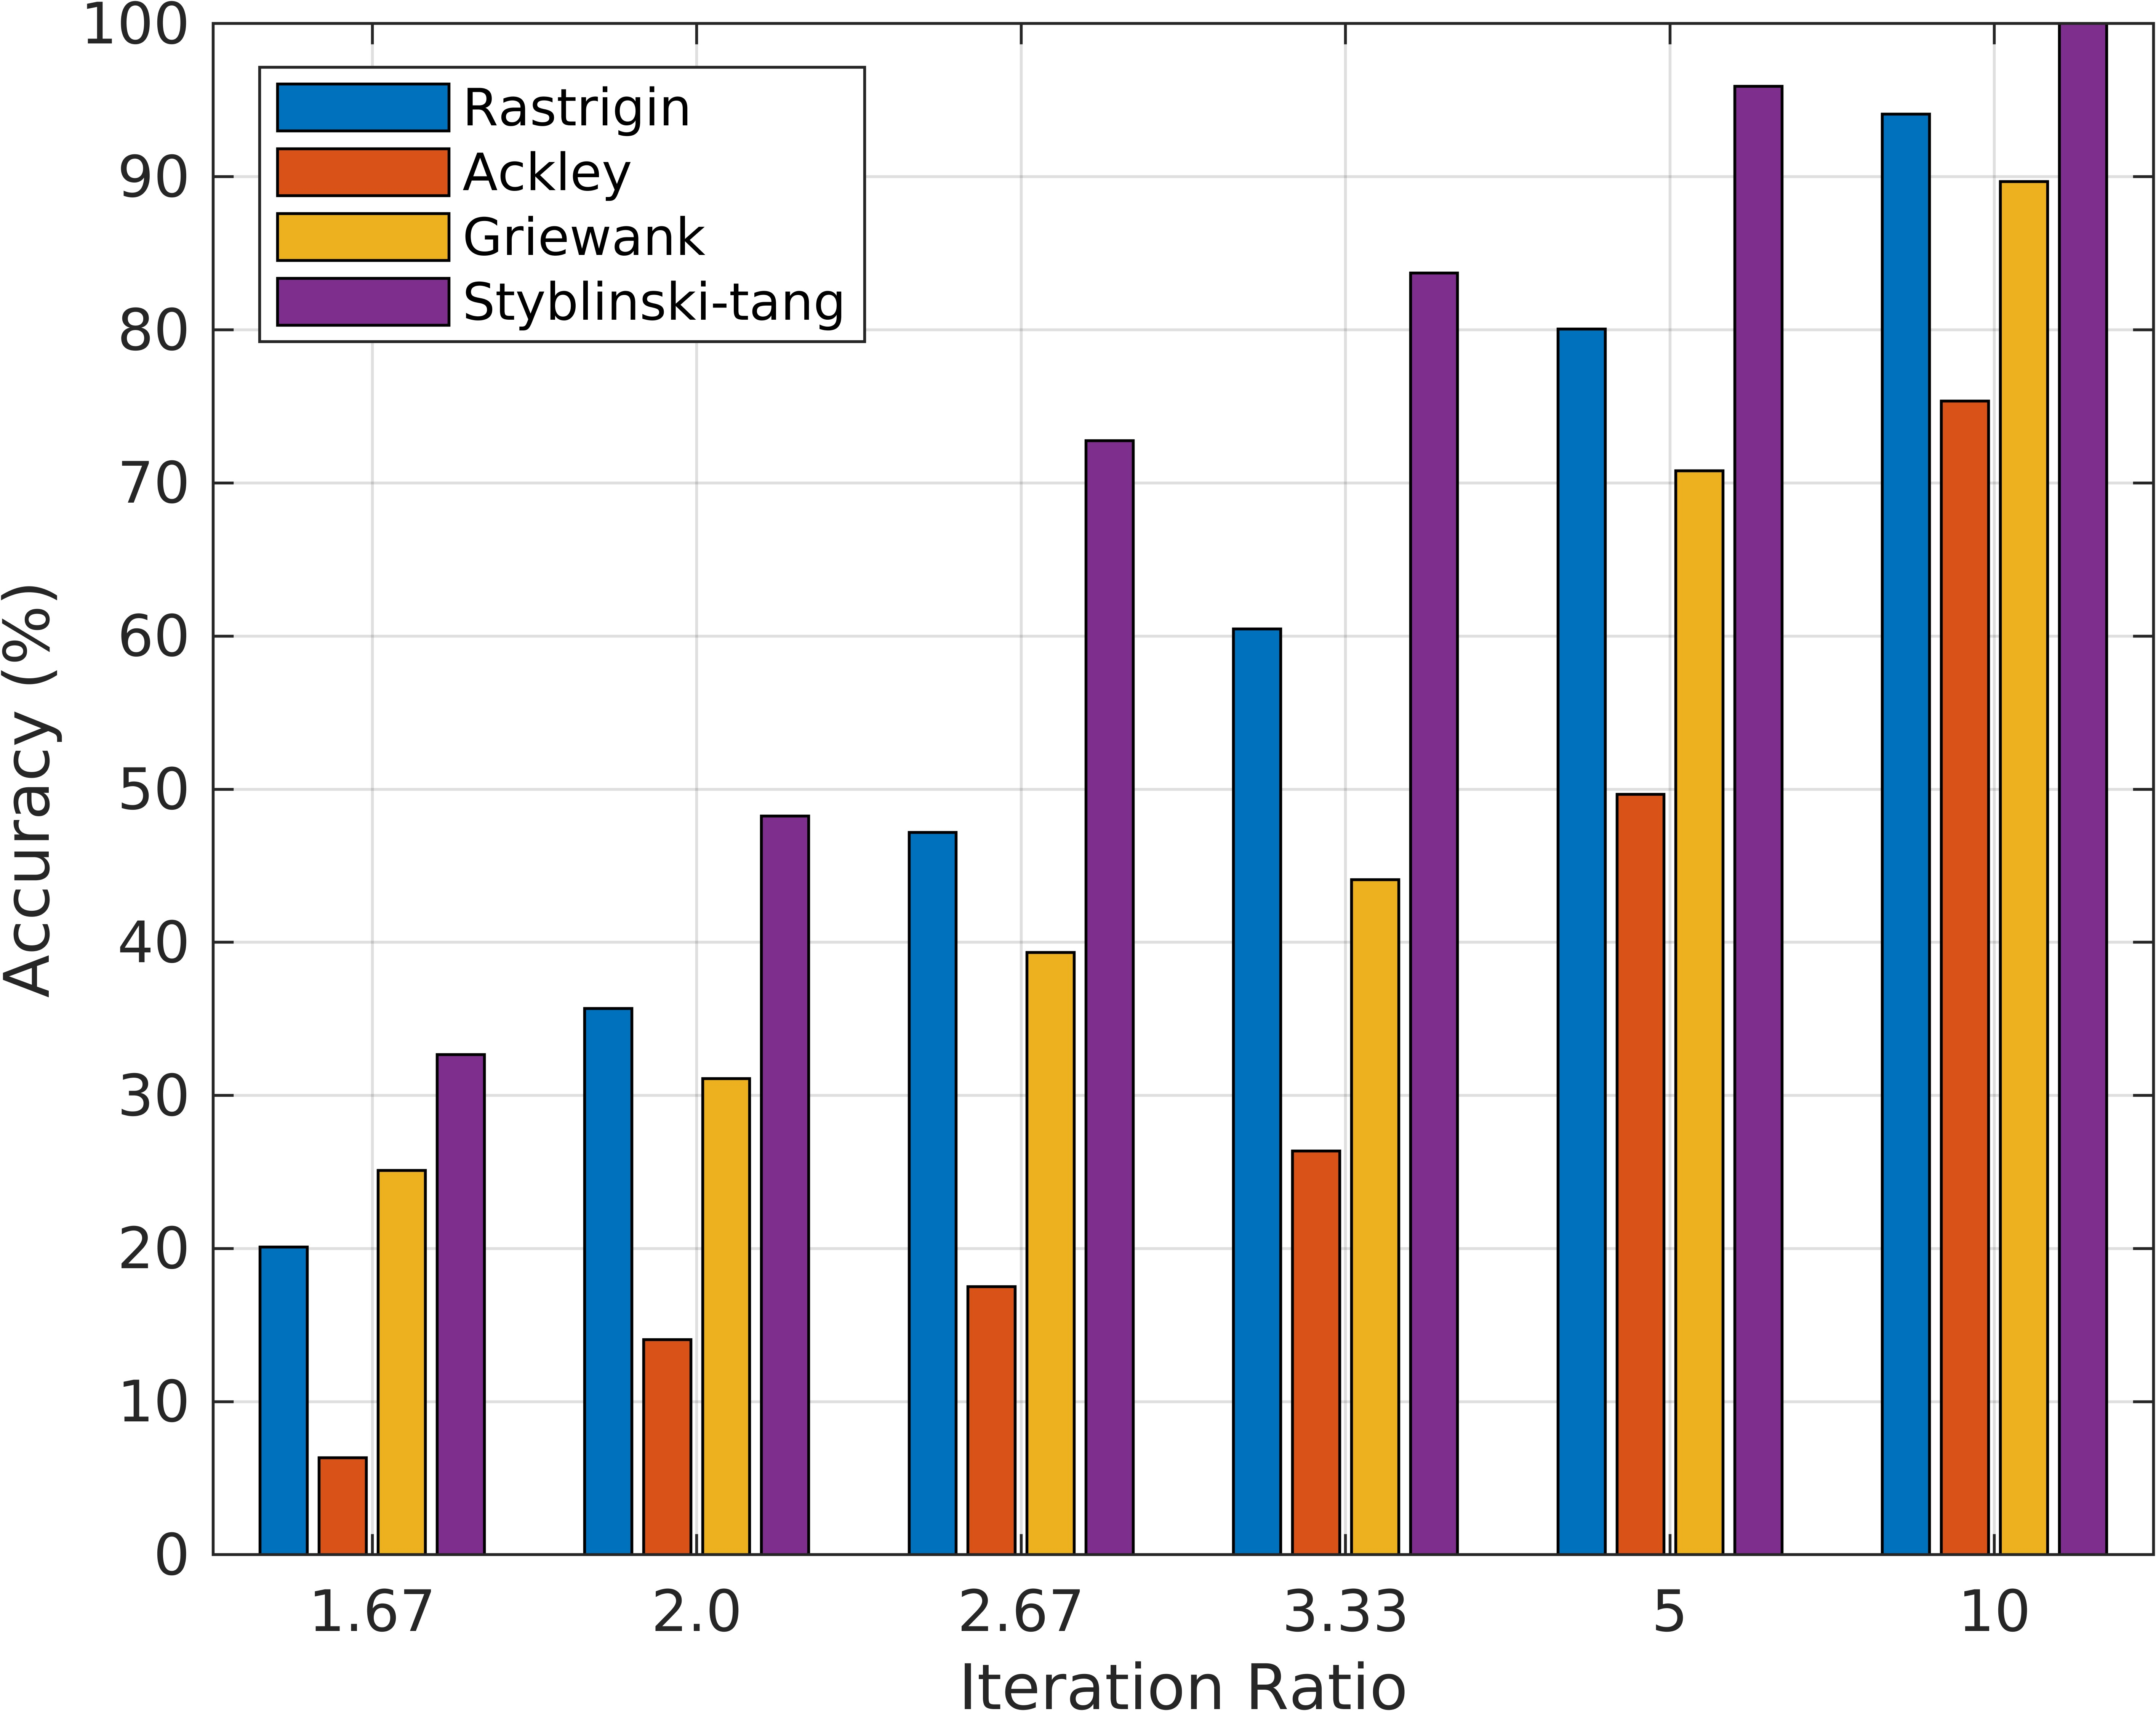
\includegraphics[width=0.8\paperwidth]{Fig/iteration_vs_accuracy.jpeg}
%		\caption{Accuracy variation with iterations keeping the swarm size at 30 for all test functions.}
%		\label{fig:acc_itr}
%	\end{figure}
	
	\item Acuuracy with swarm size: In this study, accuracy is evaluated across all tests by varying the swarm size, starting with 30 particles and increasing it by factors of 1.67, 2.0, 2.67, 3.00, 5, and 10, while keeping the number of iterations constant at 1000. The findings indicate that as the swarm size increases, accuracy improves to approximately 70 \%.
\end{enumerate}
From these experiments for finding the optimization parameters, it is concluded that an optimal combination of inertia weights between 0.5 and 0.8, \(c_1\) values ranging from 0.6 to 2.0, and \(c_2\) values between 0.6 and 1.8 leads to enhanced accuracy. Additionally, increasing the number of iterations relative to the number of particles is beneficial, as it provide improved accuracy while maintaining similar computational costs.
\\
The parameters that performed well in the previous experiments with test functions are used to evaluate the rate of convergence for the Schwefel function, as shown in figure \ref{fig:schwefel}. This additional test function focuses solely on the objective function with respect to the number of iterations, as illustrated in figure \ref{fig:con_schwefel}. The aim of this study is to identify a combination of optimization parameters that achieve a better rate of convergence, enabling optimized results to be obtained within fewer iterations. Figure \ref{fig:con_schwefel} illustrates that higher values of inertia do not show convergence, while lower values of inertia exhibit a high rate of convergence but fail to reach the optimized value. An inertia value of 0.6 demonstrates good convergence with different \(c_1\) and \(c_2\) values. This analysis reveals that \(c_1\) at 1.8 and \(c_2\) at both 1.8 and 2.4 converge to zero, albeit slowly. In contrast, \(c_1\) at 2.4 and \(c_2\) ranging from 1.2 to 1.8 exhibit a good rate of convergence, reaching near zero within 100 iterations. Based on this analysis, the optimal parameters for further seismic inversion are set as inertia at 0.6, \(c_1\) at 2.4, and \(c_2\) between 1.2 and 1.8.
%\begin{figure}	
%	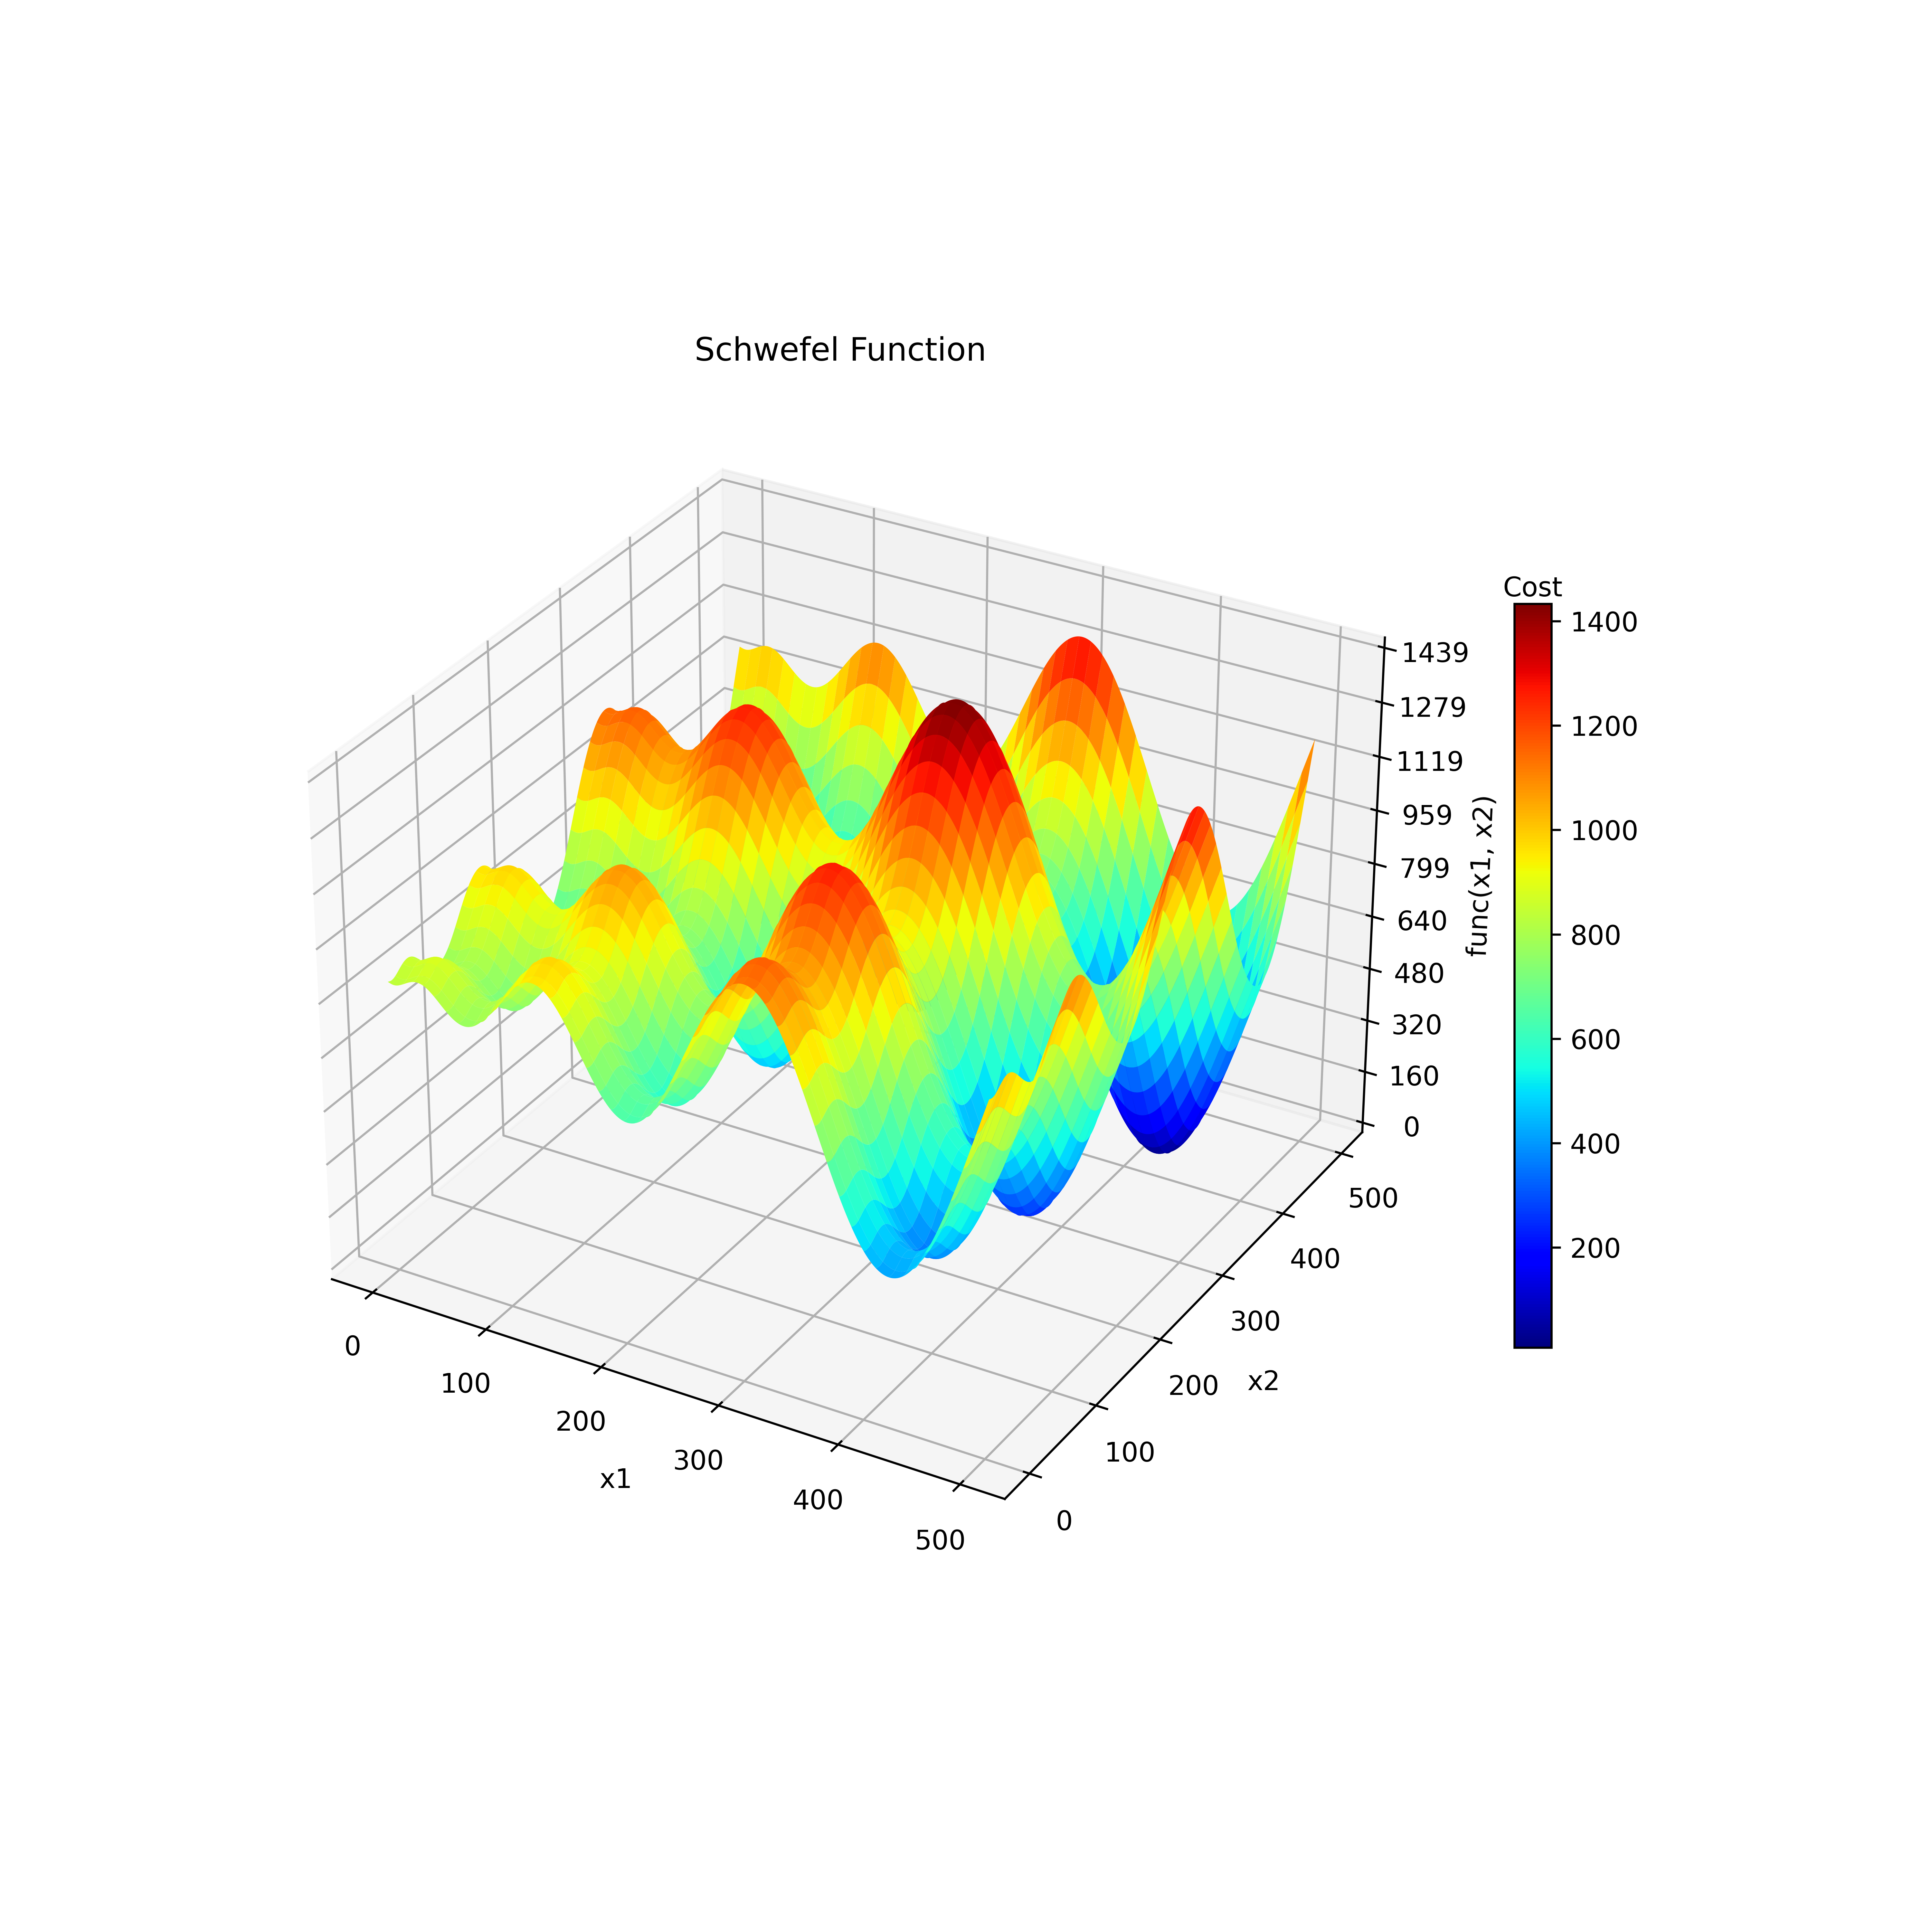
\includegraphics[width=0.8\paperwidth]{Fig/schwefel.png}
%	\caption{Schwefel function.}
%	\label{fig:schwefel}
%\end{figure}

%\begin{figure}	
%	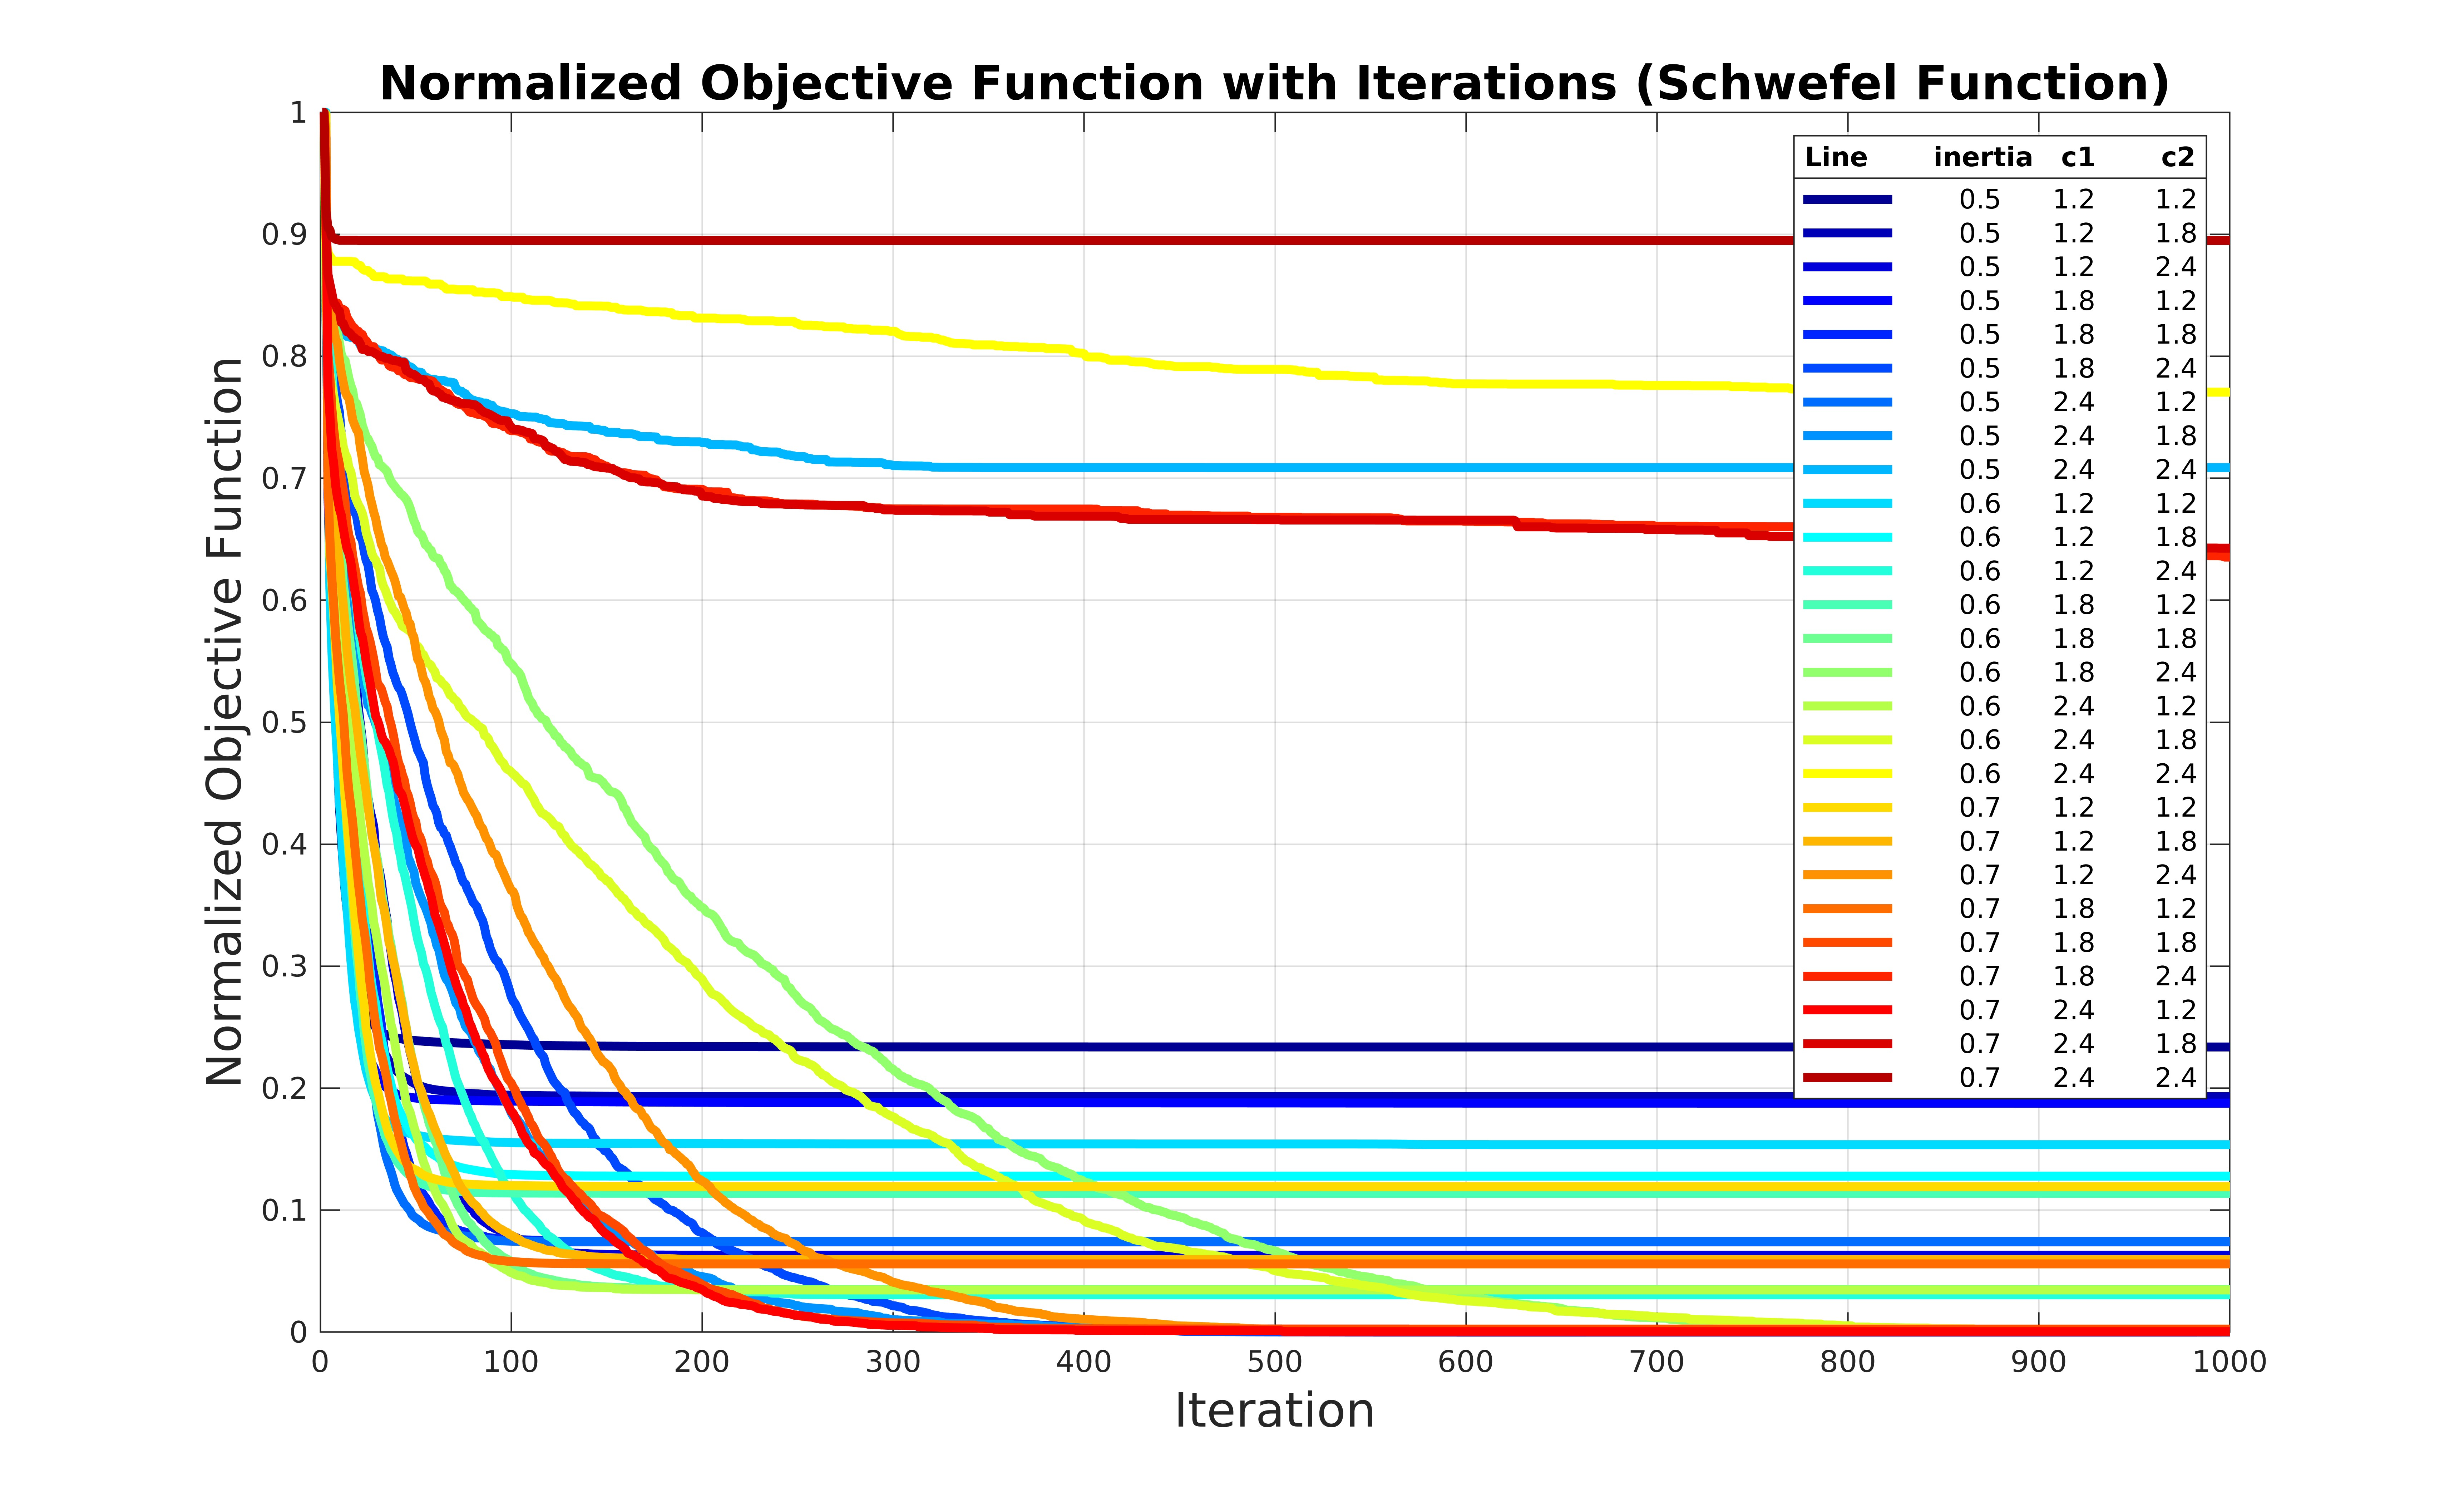
\includegraphics[width=0.8\paperwidth]{Fig/con_vs_itr.jpg}
%	\caption{Objective function versus iteration for Schwefel function.}
%	\label{fig:con_schwefel}
%\end{figure}

\subsection{Model Parameterization}
The seismic model includes physical parameters defined at densely packed grid points, often in the thousands, leading to an exponentially expanding search space that complicates the implementation of PSO. Therefore, it is essential to create a method for defining these velocity models with fewer parameters before implementing PSO, ensuring that the resulting output model can effectively serve as an initial model for FWI. 
\\
We propose a technique to define model with depth-velocity profile at sparse horizontal positions, as illustrated in Figure \ref{fig:parameterization.jpg}. This model represents a layered marine environment, where the velocity gradually increases with depth, ranging from 1500 to 4700 m/s. Additionally, it features a low-velocity layer situated between two high-velocity layers. The depth of interfaces (\(c_i^k\)), where \(i\) represents the \(i^{th}\) interface for the \(k^{th}\) depth-velocity profile, (\(g_i^k\)) denotes the rate of change of velocity between the \((i - 1)^{th}\) and \(i^{th}\) interfaces, and (\(v_i^k\)) indicates the velocity of the model at the \(i^{th}\) interface.  These multiple, sparsely located depth-velocity profiles are interpolated using cubic splines to create an initial model. It is assumed that no two interfaces intersect, as this is geologically implausible. Furthermore, the search space is restricted to feasible physical parameters. With these constraints, PSO is employed to optimize the three parameters for each layer in the development of the initial model.

%\begin{figure}	
%	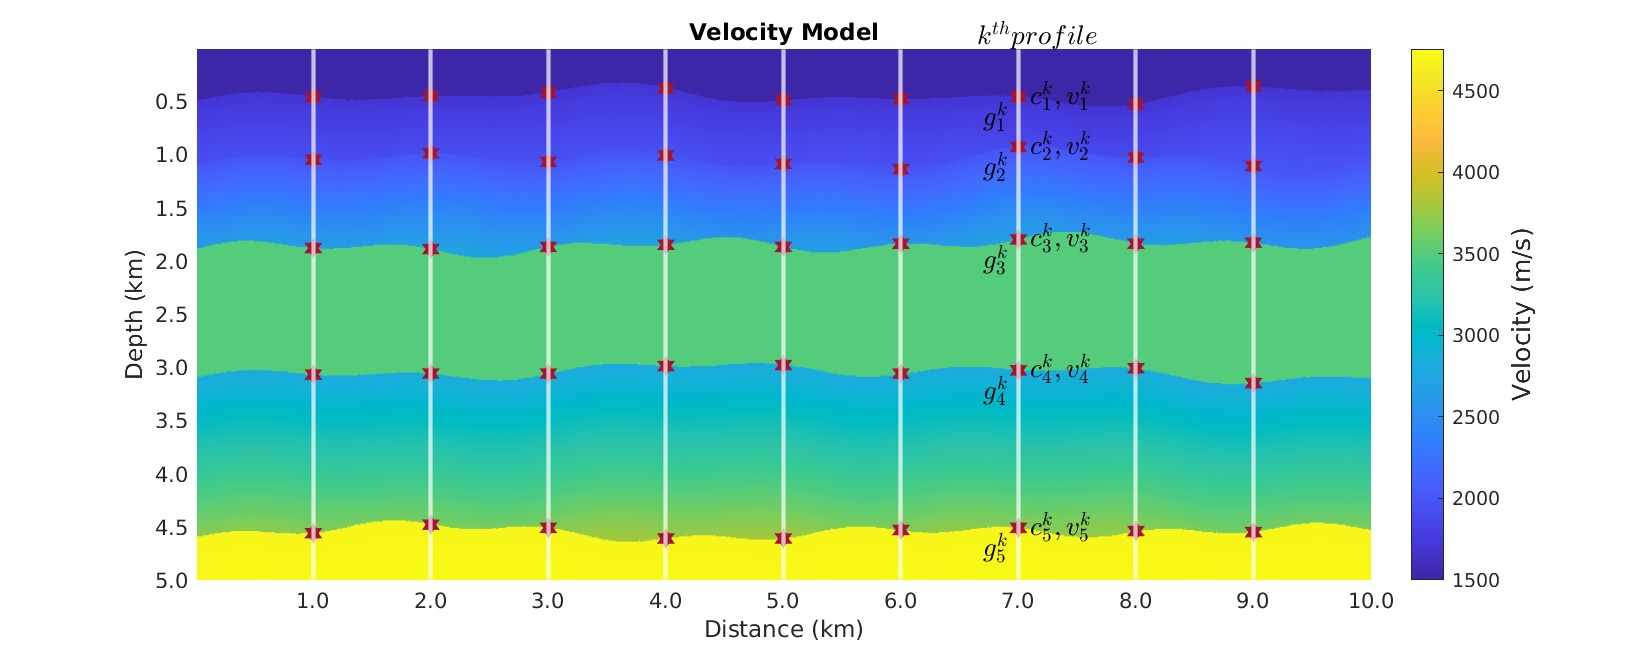
\includegraphics[width=0.8\paperwidth]{Fig/parameterization.jpg}
%	\caption{layered model.}
%	\label{fig:parameterization}
%\end{figure}

\subsection{Implementation}
The workflow of this implementation is illustrated in Figure \ref{fig:work_flow}. It shows that initial model preparation begins with a uniform 1D depth-velocity profile as the initial model, where the velocity is same as upper layer and three parameters—depth, velocity at the interface, and the rate of change of velocity—are used as input parameters initially which are set to zero. A synthetic trace for this model is generated and compared to the observed data using the L2 norm, as described by equation \ref{eqn:l2norm}.
The observed data consists only near-offset data, where the major peaks are likely caused by reflectors directly beneath the shot location. These major peaks are selected from the observed data to guide the inversion process, focusing on inverting the major reflectors progressively. The inverted model justifying a particular peak used as an initial model for the next one. This process is repeated until the inversion successfully accounts for all the selected peaks for a shot. We allow flexibility in the timing of the selected peaks since it is not always precise to pinpoint the exact peak. The peaks resulting from multiples will not significantly impact the model because the interfaces causing these multiples have already been accounted.
We sparsely select the shot locations and repeat this process for all chosen shots. Using the inverted reflectors from these shots, we create an initial model through cubic spline interpolation and smoothing. This serves as the initial model for FWI.

%\begin{figure}	
%	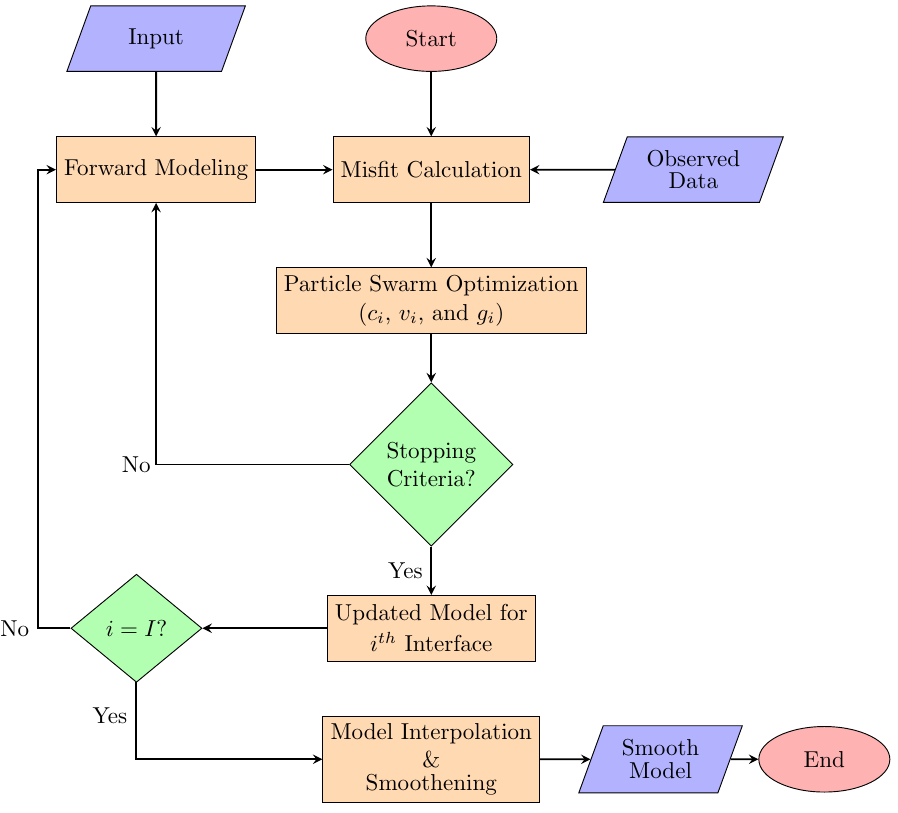
\includegraphics[width=0.5\paperwidth]{Fig/flow_chart.png}
%	\caption{Work-flow.}
%	\label{fig:work_flow}
%\end{figure}

\begin{equation}
	O(syn^k, obs^k) = \sqrt{\sum_{i=1}^{N} \left( syn^k - obs^k \right)^2}
	\label{eqn:l2norm}
\end{equation}

Where \(obs^k\) and \(syn^k\) indicate the observed data and synthetic data generated from the model, respectively; \(k\) refers to the shot number, and \(N\) represents the total samples.

\subsection{Full Waveform Inversion}

\section*{Theory}

This is another section. 

\subsection{Equations}

Section headings should be capitalized. Subsection headings should
only have the first letter of the first word capitalized.

Here are examples of equations involving vectors and tensors:
\begin{equation}
\tensor{R} = 
\pmatrix{R_{\rs{XX}} & R_{\rs{YX}} \cr R_{\rs{XY}} & R_{\rs{YY}}} 
=
\tensor{P}_{M\rightarrow R} \; \tensor{D} \; \tensor{P}_{S\rightarrow M}
\;\;\; \tensor{S} \ \ \  ,
\label{SVD}
\end{equation}
and
\begin{equation}
R_{j,m}(\omega) =
\sum_{n=1}^{N} \, \,
P_{j}^{(n)}(\mathbf{x}_R) \, \,
D^{(n)}(\omega) \, \,
P_{m}^{(n)}(\mathbf{x}_S) \ \ \ .
\label{SVDray}
\end{equation}
\ref{SVDray}
Note that the macro for the \verb#\tensor# command has been changed to
force tensors to be bold uppercase, in compliance with current SEG
submission standards. This is so that documents typeset to the old
standards will print out according to the new ones: e.g., tensor
$\tensor{t}$ (note converted to uppercase).

\subsection*{Figures}
\renewcommand{\figdir}{Fig} % figure directory

Figure~\ref{fig:waves} shows what it is about.

\plot{waves}{width=\textwidth}
{This figure is specified in the document by \texttt{
    $\backslash$plot\{waves\}\{width=$\backslash$textwidth\}\{This caption.\}}.
}

\subsubsection{Multiplot} 


The first argument of the \texttt{multiplot} command specifies the
number of plots per row.

\subsection{Tables}


\begin{acknowledgments}
I wish to thank Ivan P\v{s}en\v{c}\'{\i}k and Fr\'ed\'eric Billette
for having names with non-English letters in them.  I wish to thank
\cite{Cerveny} for providing an example of how to make a bib file that
includes an author whose name begins with a non-English character and
\cite{forgues96} for providing both an example of referencing a Ph.D.
thesis and yet more non-English characters.
\end{acknowledgments}

\append{Appendix example}
\label{example}

According to the new SEG standard, appendices come before references.

\begin{equation}
\frac{\partial U}{\partial z} = 
\left\{
  \sqrt{\frac{1}{v^2} - \left[\frac{\partial t}{\partial g}\right]^2} +
  \sqrt{\frac{1}{v^2} - \left[\frac{\partial t}{\partial s}\right]^2}
\right\}
\frac{\partial U}{\partial t}
\label{eqn:partial}
\end{equation}
It is important to get equation~\ref{eqn:partial} right. See also
Appendix~\ref{equations}.

\append[equations]{Another appendix}

\begin{equation}
\frac{\partial U}{\partial z} = 
\left\{
  \sqrt{\frac{1}{v^2} - \left[\frac{\partial t}{\partial g}\right]^2} +
  \sqrt{\frac{1}{v^2} - \left[\frac{\partial t}{\partial s}\right]^2}
\right\}
\frac{\partial U}{\partial t}
\label{eqn:partial2}
\end{equation}
Too lazy to type a different equation but note the numeration.

The error comparison is provided in Figure~\ref{fig:errgrp}.

\sideplot{errgrp}{width=0.8\textwidth}
{This figure is specified in the document by \texttt{
    $\backslash$sideplot\{errgrp\}\{width=0.8$\backslash$text\-width\}\{This caption.\}}.
}

\append{The source of this document}

\verbatiminput{geophysics_paper.tex}

\append{The source of the bibliography}

\verbatiminput{geophysics_reference.bib}

\newpage

\bibliographystyle{seg}  % style file is seg.bst
\bibliography{geophysics_reference}

\end{document}
